% Localização, localização, localização: um modelo de fundação tabular precisa de
% atributos espaciais? — versão em português do manuscrito. Compilar:
%   pdflatex "Localização, localização, localização - um modelo de fundação tabular precisa de atributos espaciais"
%   bibtex   "Localização, localização, localização - um modelo de fundação tabular precisa de atributos espaciais"
%   pdflatex (mais duas vezes)
% Todos os números são lidos dos resultados versionados em ../results/ e ../data/ e
% conferidos por paper/check_numbers.py (os mesmos valores da versão em inglês,
% grafados com vírgula decimal).
\documentclass[11pt,a4paper]{article}
\usepackage[margin=2.5cm]{geometry}
\usepackage[utf8]{inputenc}
\usepackage[T1]{fontenc}
\IfFileExists{portuges.ldf}{\usepackage[brazilian]{babel}}{%
  \AtBeginDocument{%
    \renewcommand{\figurename}{Figura}\renewcommand{\tablename}{Tabela}%
    \renewcommand{\refname}{Refer\^encias}\renewcommand{\abstractname}{Resumo}%
    \renewcommand{\appendixname}{Ap\^endice}}}
\IfFileExists{lmodern.sty}{\usepackage{lmodern}}{}
\usepackage[expansion=false]{microtype}
\usepackage{amsmath,amssymb}
\usepackage{booktabs}
\usepackage{graphicx}
\usepackage{caption}
\usepackage{subcaption}
\usepackage{xcolor}
\usepackage{url}
\usepackage[hidelinks]{hyperref}
\usepackage[numbers,sort&compress]{natbib}
\graphicspath{{figures/}}
\captionsetup{font=small,labelfont=bf}
\setlength{\bibsep}{2.5pt plus 0.3ex}
\setlength{\textfloatsep}{11pt plus 2pt minus 3pt}
\setlength{\floatsep}{9pt plus 2pt minus 2pt}
\setlength{\emergencystretch}{2.2em}
\newcommand{\Rsqm}{R\$/m\textsuperscript{2}}

\title{Localização, localização, localização: um modelo de fundação tabular precisa de
atributos espaciais?\\
\large O TabPFN-3.5 contra a econometria espacial e o \emph{gradient boosting} em 130.000
preços de transação declarados em São Paulo}

\author{Agnaldo Calvi Benvenho\thanks{IBAPE Nacional (Instituto Brasileiro de Avaliações e
Perícias de Engenharia) e Universidade Presbiteriana Mackenzie, São Paulo, Brasil.
\texttt{agnaldo.benvenho@gmail.com}. Código e dados:
\url{https://github.com/abenvenho/tabpfn-itbi-sp}.}}
\date{Outubro de 2026}

\begin{document}
\maketitle

\begin{abstract}
\noindent Os modelos de avaliação em massa codificam explicitamente a
dependência do preço em relação à localização, por meio de matrizes de pesos espaciais,
defasagens espaciais, modelos locais geograficamente ponderados ou atributos de vizinhança
construídos à mão. Este trabalho pergunta se um modelo de fundação tabular pode dispensar tudo
isso. O TabPFN-3.5 recebe os atributos do imóvel e as coordenadas geográficas como duas colunas
numéricas comuns, sem nenhuma modelagem espacial, e é comparado com um modelo hedônico por
OLS, um modelo autorregressivo espacial de defasagem (SAR, estimação GM), um XGBoost com
defasagem espacial de $k$ vizinhos mais próximos, coordenadas rotacionadas e ajuste aninhado, e
um XGBoost geograficamente ponderado. Os dados são 82.187 preços de transação declarados do
imposto de transmissão de São Paulo (ITBI) em 2025 e 47.810 nos sete primeiros meses de 2026,
para apartamentos, casas e unidades comerciais. A avaliação tem duas pernas: validação cruzada
deixando de fora um dos dez blocos espaciais por vez, e um teste fora do tempo que ajusta em
2025 e prevê 2026. Os critérios de refutação foram fixados antes das rodadas: erro agregado
pior, derrotas na maioria dos blocos sob testes pareados, ou mais autocorrelação espacial
residual ($I$ de Moran) que a deixada pelas \emph{baselines} explicitamente espaciais. Fora do
tempo, o modelo de tabela crua vence os três especialistas espaciais em ao menos 9 dos 10
blocos (RMSE de 0,265 no logaritmo do valor unitário contra 0,283--0,326; MAPE de 19,5\%
contra 20,9--25,0\%) e deixa a menor autocorrelação residual entre os modelos comparados
($I = 0{,}092$); com o CEP bruto no lugar das coordenadas --- uma coluna de texto, nenhuma
geometria --- todos esses vereditos se mantêm. Nos blocos nunca vistos, empata com as duas
variantes de XGBoost no erro e vence o SAR, mas deixa mais estrutura espacial nos resíduos
($I = 0{,}348$ contra 0,309--0,326): refutação parcial, registrada. O SHAP por permutação
mostra as duas coordenadas como os insumos mais fortes do modelo; o resultado do CEP mostra
que, dentro de um mercado observado, o que elas carregam é a localização como identificador, e
não geometria, e que só coordenadas extrapolam para distritos sem vendas. Para a avaliação em
massa dentro de um mercado com histórico de vendas, o modelo de fundação com a tabela crua é o
preditor mais forte desta comparação, com um único ajuste de quinze segundos e nenhuma
engenharia espacial.

\medskip
\noindent\textbf{Palavras-chave:} avaliação em massa; modelos de fundação tabulares; TabPFN;
autorregressão espacial; validação cruzada espacial; preços hedônicos; São Paulo.
\end{abstract}

\section{Introdução}
\label{sec:intro}

A avaliação em massa na escala da cidade apoia-se na leitura hedônica do mercado imobiliário
\citep{rosen1974}: o preço de um bem heterogêneo é função de seus atributos, e a localização é
o atributo que domina os demais --- coisas próximas são mais relacionadas que coisas distantes
\citep{tobler1970}. Os preços de imóveis vizinhos não são, portanto, observações independentes,
o que fere a hipótese por trás da regressão por mínimos quadrados ordinários em que a prática
de avaliação se apoia \citep{anselin1988}. As respostas consagradas modelam a dependência de
forma explícita: uma matriz de pesos espaciais e um termo autorregressivo na econometria
espacial \citep{anselin1988,lesage2009}, modelos locais reajustados ao longo do mapa na
regressão geograficamente ponderada \citep{fotheringham2002} e em seus descendentes baseados em
árvores \citep{grekousis2025}, ou atributos de vizinhança alimentados à mão a um
\emph{gradient boosting}. Tudo isso funciona --- e tudo isso é engenharia que precisa ser
refeita para cada cidade e cada base: uma matriz de pesos a construir, uma banda a calibrar,
uma defasagem a recalcular dentro de cada dobra de treino.

Os modelos de fundação para dados tabulares oferecem outro contrato. O TabPFN é um
\emph{transformer} \citep{vaswani2017} pré-treinado em milhões de tarefas tabulares sintéticas;
no uso, realiza aprendizado em contexto: toma a tabela de treino inteira como entrada e prevê
as linhas de teste em uma única passagem, sem passos de gradiente e sem ajuste
\citep{hollmann2023tabpfn,hollmann2025nature}. A terceira geração estendeu a abordagem a
tabelas grandes e à regressão \citep{priorlabs2026tabpfn3}, e a versão 3.5 lê nativamente
colunas categóricas de alta cardinalidade e texto livre \citep{priorlabs2026tabpfn35}. Se um
modelo assim, recebendo latitude e longitude como duas colunas numéricas simples, aprende a
dependência espacial que os especialistas codificam por construção é uma pergunta empírica em
aberto --- e prática, porque, se aprende, a maquinaria espacial acima se torna opcional para
uma classe ampla de problemas de avaliação.

A pergunta tem origem concreta. Em um estudo comparativo sobre 5.005 ofertas de apartamentos em
Belo Horizonte, o TabPFN v3 com coordenadas cruas superou OLS, SAR, SEM e um modelo
semiparamétrico de defasagem espacial sob validação cruzada por blocos espaciais
\citep{benvenho2026cead}. Aquele resultado pedia um teste mais duro, e este artigo é esse
teste: preços de transação declarados em vez de ofertas, três tipologias em vez de uma, 82.187
linhas de treino em vez de 5.005, uma perna de um ano à frente somada à validação por blocos,
um critério de autocorrelação residual capaz de refutar a tese mesmo onde o erro não refuta, e
um conjunto mais forte de oponentes espaciais. O enquadramento é falsificacionista: a hipótese
é enunciada antes das rodadas, com os critérios que a refutariam, e a comparação é
deliberadamente assimétrica \emph{contra} ela --- as \emph{baselines} mantêm todas as vantagens
espaciais, o modelo de fundação recebe a tabela crua.

A hipótese é enunciada de modo que possa falhar:

\begin{quote}
Um modelo de fundação tabular que recebe apenas os atributos do imóvel e as coordenadas como
duas colunas numéricas simples --- sem matriz de pesos espaciais, sem defasagem espacial, sem
atributos de vizinhança construídos à mão --- prevê preços espacialmente correlacionados tão
bem quanto, ou melhor que, modelos especializados que codificam a dependência espacial
explicitamente.
\end{quote}

Ela é refutada se qualquer um dos itens a seguir valer sob um protocolo comum: RMSE ou MAPE
agregados piores; derrotas na maioria dos blocos espaciais sob testes pareados; ou mais
autocorrelação espacial deixada nos resíduos fora da amostra do que a deixada pelos modelos
explicitamente espaciais.

O artigo contribui com: (i) uma comparação de um modelo de fundação tabular com
\emph{baselines} de econometria espacial e de árvores espacialmente aumentadas --- entre elas
um XGBoost geograficamente ponderado --- sobre preços declarados na escala da cidade; (ii) um
protocolo de duas pernas, validação cruzada por blocos espaciais mais teste fora do tempo, com
critérios de refutação pré-registrados que incluem a autocorrelação espacial residual; (iii)
ablações que isolam o que carrega a localização dentro do modelo, substituindo as coordenadas
por um CEP bruto e acrescentando o texto livre do formulário do imposto; (iv) um
\emph{pipeline} público e reproduzível sobre dados municipais abertos; e (v) o próprio achado,
refutação parcial incluída.

\section{Trabalhos relacionados}
\label{sec:related}

\paragraph{Modelos hedônicos espaciais.} O arcabouço hedônico \citep{rosen1974} combinado com a
primeira lei de Tobler \citep{tobler1970} leva à família da econometria espacial: os modelos de
defasagem espacial (SAR) e de erro espacial, estimados por máxima verossimilhança ou pelo
procedimento de momentos generalizados de \citet{kelejian1998}, com a matriz de pesos como
portadora da estrutura de vizinhança \citep{anselin1988,lesage2009}. A regressão
geograficamente ponderada abandona o vetor global de coeficientes e reajusta um modelo local em
cada ponto de calibração, com pesos decrescentes na distância \citep{fotheringham2002}.

\paragraph{Aprendizado de máquina com atributos espaciais.} Os conjuntos de árvores não
enxergam o espaço, a menos que ele lhes seja servido. Os dispositivos usuais são a defasagem
espacial da resposta calculada sobre os vizinhos de treino, transformações de coordenadas como
eixos oblíquos ou rotacionados \citep{moller2020} e covariáveis de distância. O
Geographical-XGBoost \citep{grekousis2025} transplanta a ideia geograficamente ponderada para o
\emph{gradient boosting}: um XGBoost local por ponto de calibração, combinado com um modelo
global. Avaliar qualquer dessas alternativas com honestidade exige validação cruzada espacial,
pois partições aleatórias deixam vizinhos do ponto de teste dentro do conjunto de treino
\citep{roberts2017,meyer2022}.

\paragraph{Modelos de fundação tabulares, e o espaço dentro deles.} O TabPFN
\citep{hollmann2023tabpfn,hollmann2025nature} e sua terceira geração
\citep{priorlabs2026tabpfn3,priorlabs2026tabpfn35} substituem o treinamento por base de dados
pelo aprendizado em contexto sobre \emph{priors} sintéticos. Duas linhas recentes levam o
espaço \emph{para dentro} do modelo: o TabPFN-GSA modifica a arquitetura com atenção esparsa
geoespacial \citep{deng2026gsa}, e a \emph{Kriging-prior Regression} alimenta o TabPFN com
atributos derivados de krigagem \citep{schmidinger2026kpr}. Este artigo toma a posição oposta:
o modelo tal como distribuído, sem alteração de arquitetura e sem atributo espacial, com a
dependência deixada para o aprendiz em contexto encontrar em duas colunas cruas.

\paragraph{TabPFN na avaliação de imóveis.} Até onde o autor conhece, as únicas aplicações
publicadas do TabPFN à avaliação de imóveis são as suas próprias, ambas em português. Sobre
preços de transação do ITBI de São Paulo, o TabPFN v2 superou um FT-Transformer e a regressão
linear múltipla \citep{benvenho2026igel}; sobre as ofertas de Belo Horizonte, o TabPFN v3
superou os modelos econométricos espaciais, lineares e não lineares, da comparação
\citep{benvenho2026cead}. Em relação a este último, o presente estudo muda a resposta (preços
declarados em vez de ofertas), o escopo (três tipologias em vez de apenas apartamentos), a
escala (82.187 linhas de treino em vez de 5.005), o protocolo (acrescenta a perna fora do tempo
e o critério de autocorrelação residual) e os oponentes (um XGBoost espacialmente aumentado e
um XGBoost geograficamente ponderado somam-se às \emph{baselines} econométricas).

\section{Dados}
\label{sec:data}

\subsection{Fonte e saneamento}

A Prefeitura de São Paulo publica todas as guias pagas do imposto de transmissão de bens
imóveis (ITBI) com o preço de transação declarado, a chave cadastral (SQL: setor, quadra, lote)
e os atributos físicos do imóvel vindos do cadastro do IPTU: áreas construída e de terreno,
uso, padrão construtivo, ano de construção corrigido. O arquivo de 2025 contém 230.525 guias e
o de janeiro--julho de 2026, 135.655. As coordenadas vêm dos centroides dos polígonos de quadra
fiscal do cadastro municipal (GeoSampa), de modo que todos os imóveis de uma mesma quadra
compartilham a localização; a distância à estação de metrô ou trem mais próxima é calculada a
partir dos 203 pontos de estação do mesmo portal.

A Tabela~\ref{tab:filters} apresenta a cadeia de saneamento com a contagem de registros após
cada passo; o relatório completo, aberto por tipologia, está versionado com os dados
(\texttt{data/filter\_report.md}). As bases limpas contêm 82.187 transações de 2025 (treino) e
47.810 de 2026 (teste). Uma amostra estratificada de 24.000 linhas de 2025 (12.000
apartamentos, 7.000 casas, 5.000 unidades comerciais; ``Nível~A'') é usada onde as
\emph{baselines} mais lentas precisam rodar.

\begin{table}[t]
\centering\small
\caption{A cadeia de saneamento: registros remanescentes após cada passo.}
\label{tab:filters}
\footnotesize
\begin{tabular}{clrr}
\toprule
\# & Passo & 2025 & 2026 (jan--jul) \\
\midrule
0 & Base bruta (todas as guias pagas de ITBI) & 230.525 & 135.655 \\
1 & Natureza da transação contém ``compra e venda'' & 207.518 & 124.289 \\
2 & Proporção transmitida $= 100\%$ & 108.750 & 61.304 \\
3 & Situação cadastral ativa & 108.420 & 61.112 \\
4 & SQL válido de 11 dígitos e data válida & 108.420 & 61.112 \\
5 & Tipologia mantida (apartamento / casa / comercial) & 90.927 & 51.919 \\
6 & Área construída (de referência) $> 0$ & 90.927 & 51.919 \\
7 & ACC plausível ($1900 \le \text{ACC} \le$ ano da transação) & 90.927 & 51.918 \\
8 & Deduplicação em (chave, data, preço) & 90.673 & 51.810 \\
9 & Preço declarado $\ge$ R\$ 10.000 & 89.078 & 51.202 \\
10 & Razão preço / valor venal de referência em $[0{,}3,\ 5]$ & 87.488 & 50.430 \\
11 & Subdeclaração: excluídas as compras à vista coladas no VVR & 84.263 & 48.879 \\
12 & Cercas de Tukey ($1{,}5$ IQR) em $\ln(\text{\Rsqm})$, por tipo (cercas de 2025) & 82.193 & 47.814 \\
13 & Junção ao centroide da quadra fiscal (99,99\%) & 82.187 & 47.810 \\
\bottomrule
\end{tabular}
\end{table}

\subsection{Subdeclaração}

A base de cálculo do ITBI é $\max(\text{preço declarado},\ \text{valor venal de referência})$,
de modo que quem subdeclara não tem incentivo a declarar abaixo do valor de referência: as
compras à vista subdeclaradas acumulam-se exatamente sobre ele. O diagnóstico encontrou esse
acúmulo concentrado nas compras à vista, e o \emph{pipeline} remove as transações à vista
declaradas a menos de $1\%$ do valor de referência: 3.225 guias em 2025 e 1.551 em 2026 (passo
11 da Tabela~\ref{tab:filters}; o quadro residual após a exclusão está em
\texttt{data/underdeclaration\_report.md}). As transações financiadas passam pela análise do
credor e são mantidas; a Seção~\ref{sec:robust} repete toda a análise apenas sobre elas.

\subsection{Estatísticas descritivas}

\begin{table}[h]
\centering\small
\caption{As três bases. Valor unitário (VU) $=$ preço declarado / área construída, em \Rsqm; a última coluna é a sua mediana.}
\label{tab:data}
\footnotesize
\begin{tabular}{lrrrrrr}
\toprule
Base & Linhas & Apart. & Casas & Comercial & Financ. & Mediana do VU \\
\midrule
2025, completa (treino) & 82.187 & 60.067 & 15.940 & 6.180 & 34\% & 4.836 \\
2025, Nível A (amostra) & 24.000 & 12.000 & 7.000 & 5.000 & 30\% & 4.715 \\
2026, jan--jul (teste) & 47.810 & 35.354 & 9.429 & 3.027 & 42\% & 4.970 \\
\bottomrule
\end{tabular}
\end{table}

A resposta é fortemente autocorrelacionada no espaço, como são os preços urbanos. O $I$ de
Moran do logaritmo bruto do valor unitário, na matriz $k$-NN-8 usada em todo o artigo, é de
0,430 na amostra do Nível A ($z = 141{,}8$) e de 0,506 na base de 2026 ($z = 235{,}7$): o valor
unitário de um imóvel está próximo do de seus vizinhos muito além do acaso, exatamente a
estrutura que as \emph{baselines} espaciais foram construídas para explorar. A
Figura~\ref{fig:blocks}(a) mostra como os dez blocos espaciais recobrem essa estrutura sobre a
cidade. Como as coordenadas são centroides de quadra fiscal, a localização é resolvida na
quadra, não no endereço --- uma escolha conservadora compartilhada por todos os modelos.

\section{Métodos}
\label{sec:methods}

\subsection{Resposta e atributos}

A resposta é $y = \ln(\text{preço}/\text{área construída})$. O conjunto de informação é o mesmo
para todos os modelos: área construída, área do terreno, idade, padrão construtivo (nível do
padrão IPTU, 0--5), distância à estação mais próxima, índice do mês, tipologia, latitude e
longitude. Os modelos diferem apenas no que lhes é permitido fazer com as duas últimas.

\subsection{Modelos}

\paragraph{Hedônico por OLS.} Log-linear nas áreas e na distância, quadrático na idade,
\emph{dummies} de tipologia. As coordenadas não são covariáveis: este é o piso sem localização
da família linear.

\paragraph{SAR de defasagem.} $y = \rho W y + X\beta + \varepsilon$ com matriz de pesos de $k$
vizinhos mais próximos padronizada por linha ($k = 8$), construída dentro de cada dobra de
treino e estimada pelo procedimento de momentos generalizados de \citet{kelejian1998}, como
implementado em \texttt{spreg} \citep{rey2010pysal}. Uma linha fora da amostra é prevista pela
forma estrutural com a defasagem espacial tomada sobre seus $k$ vizinhos \emph{de treino} mais
próximos, $\hat y_i = \mathbf{x}_i^{\top}\hat\beta + \hat\rho\,\bar y_{N_8(i)}$, em que
$\bar y_{N_8(i)}$ é a média da resposta observada desses vizinhos; a forma reduzida não está
disponível fora da amostra sem a vizinhança das próprias linhas de teste, de modo que nada do
conjunto de teste entra na predição. Empates nas coordenadas de centroide são desfeitos por um
\emph{jitter} determinístico submétrico ($\pm 0{,}5$~m, semente 42), necessário porque todas as
transações de uma mesma quadra fiscal compartilham o centroide exato.

\paragraph{XGBoost com atributos espaciais.} O bloco hedônico acima mais as coordenadas UTM,
suas projeções em eixos rotacionados de $30^{\circ}$, $45^{\circ}$ e $60^{\circ}$
\citep{moller2020} e uma defasagem espacial $k$-NN-8 da resposta calculada dentro da dobra de
treino (\emph{leave-one-out} para as linhas de treino). Os hiperparâmetros são ajustados por
Optuna aninhado (30 tentativas TPE, parada antecipada, até 3.000 rodadas), com um
\emph{leave-one-block-out} interno sobre os blocos de treino; o bloco de teste externo nunca
toca o ajuste \citep{chen2016xgboost,akiba2019optuna}. Três sementes. O espaço de busca e os
valores selecionados estão no Apêndice~\ref{app:hparams}.

\paragraph{XGBoost geograficamente ponderado.} O Geographical-XGBoost \citep{grekousis2025}
ajusta um XGBoost local por ponto de calibração com pesos bi-quadrados de distância,
$w = (1 - d^2/h^2)^2$ com $h$ a distância ao $k$-ésimo vizinho, combinado com um modelo global
por $\hat y = \alpha\,\hat y_{\text{local}} + (1 - \alpha)\,\hat y_{\text{global}}$. Tal como
empacotado, ele calibra um modelo local, com sua própria busca em grade, em cada linha de
treino, sobre uma matriz densa de distâncias --- o que um piloto de viabilidade mostrou
impraticável nesta escala (Apêndice~\ref{app:gxgb}). A implementação aqui mantém o estimador e
calibra os modelos locais em 1.000 pontos de regressão --- os centros de $K$-médias das
coordenadas de treino, cerca de um por 1,5~km\textsuperscript{2} de cidade ---, como a
regressão geograficamente ponderada permite \citep{fotheringham2002}; uma localização de
consulta é prevista pela média, com pesos inversos à distância, de seus três modelos locais
mais próximos. Os modelos locais veem os atributos hedônicos e nenhuma coordenada: o espaço
entra apenas pela ponderação, como no original. A banda
$k \in \{50, 100, 200, 400, 800, 1600, 3200\} \times n_{\text{treino}}/24.000$ e a mistura
$\alpha \in \{0;\ 0{,}25;\ 0{,}5;\ 0{,}75;\ 1\}$ são escolhidas por validação cruzada interna
por blocos dentro de cada dobra externa; a grade foi ampliada para baixo, de 400 para 50,
depois que as primeiras buscas escolhiam sempre o menor valor, e 50 vizinhos é adotado como
piso. Três sementes.

\paragraph{TabPFN-3.5, tabela crua.} As nove colunas cruas, com a tipologia declarada como
categórica, pelo modelo hospedado (\texttt{tabpfn-client} 0.6.0, versão de modelo 3.5).
\emph{Zero-shot}, e uma variante em modo \emph{thinking}, na qual o ajuste explora
configurações por validação interna na dobra de treino (objetivo RMSE, esforços médio e alto).
Nenhuma informação espacial de qualquer natureza além das duas colunas de coordenadas. O ajuste
em 24.000 linhas leva cerca de 9~s; em 82.187 linhas, 15~s. Configurações no
Apêndice~\ref{app:hparams}; as variantes de entrada --- o CEP no lugar das coordenadas, o texto
livre do formulário --- são apresentadas com seus resultados na Seção~\ref{sec:carriers}.

\subsection{Protocolo de avaliação}

\paragraph{Perna 1: validação cruzada por blocos espaciais.} Dez blocos de $K$-médias sobre as
coordenadas do Nível A, cada um deixado de fora por vez \citep{roberts2017,meyer2022}. Toda
quantidade interna à dobra (matriz de pesos, defasagem espacial, ajuste, pontos de regressão) é
recalculada apenas sobre os blocos de treino. A pergunta é se o modelo consegue precificar uma
parte da cidade que nunca viu --- o teste mais duro para um modelo que se apoia na localização.

\paragraph{Perna 2: fora do tempo.} Um único ajuste em 2025 (Nível A e, depois, a base
completa), predições para todas as 47.810 transações de 2026, de um a sete meses após a janela
de treino. Nada de 2026 toca o ajuste ou a calibração. Mesma cidade, de modo que os modelos com
defasagem espacial recebem vizinhos das mesmas ruas: o cenário mais favorável à modelagem
espacial explícita. Verificação de vazamento: nenhuma transação (chave, data, preço) aparece
nos dois anos; $0{,}6\%$ das linhas de 2026 compartilham chave cadastral com o Nível A.

\paragraph{Métricas e testes.} RMSE, MAE e $R^2$ na escala logarítmica, MAPE na escala de
preço, resíduo médio (viés). Autocorrelação espacial residual pelo $I$ de Moran
\citep{moran1950} sobre a matriz $k$-NN-8 das coordenadas de teste. Comparações pareadas sobre
os dez blocos: teste de postos sinalizados de Wilcoxon exato sobre o RMSE por bloco e
\emph{bootstrap} por blocos (2.000 reamostragens de blocos) para a diferença agregada, com
intervalo percentílico de 95\%. Onde o modelo é estocástico, três sementes (42, 43, 44) e a
faixa entre sementes; uma rodada do TabPFN (semente 42) é pareada contra cada semente do
oponente estocástico.

\section{Resultados}
\label{sec:results}

\subsection{Perna 1: blocos nunca vistos}

\begin{figure}[t]
\centering
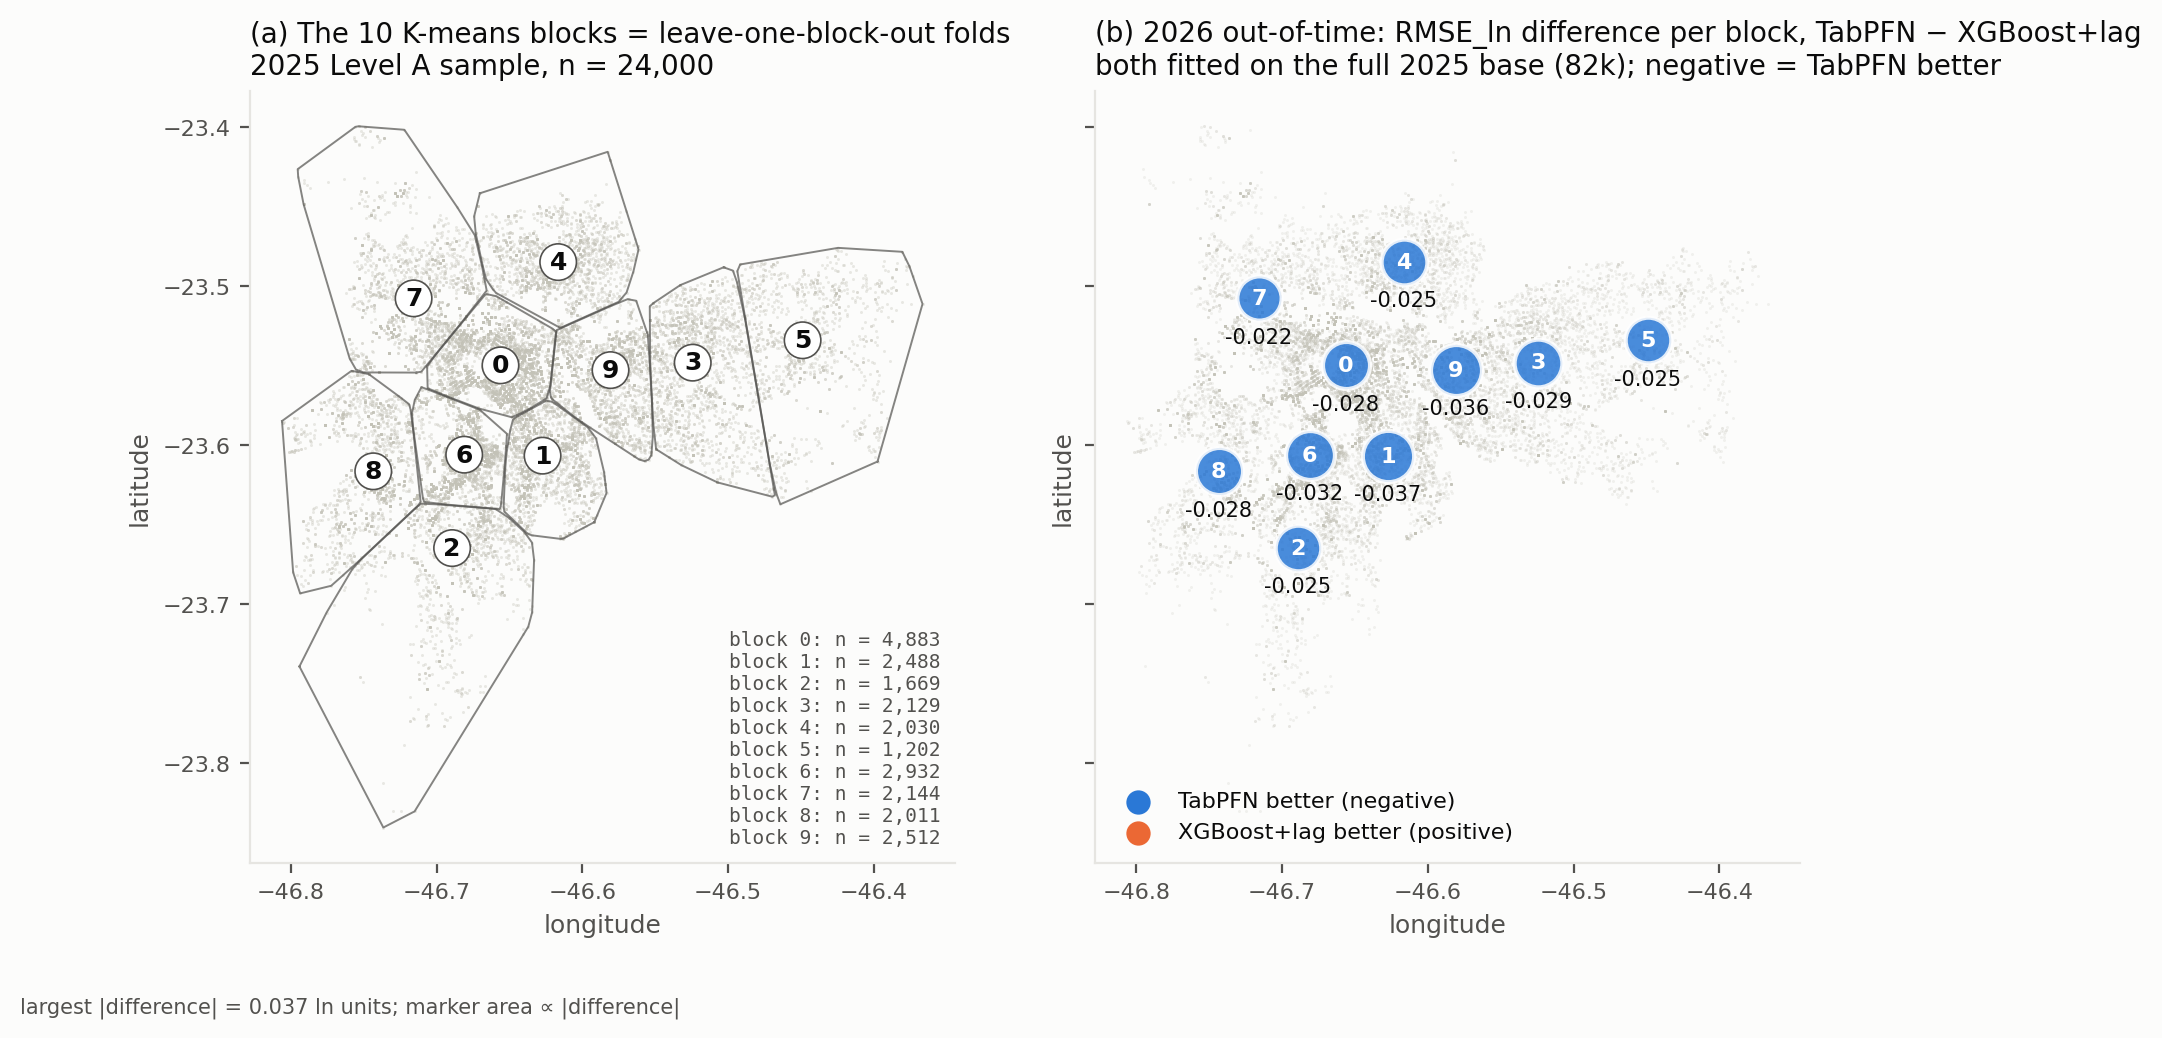
\includegraphics[width=\textwidth]{fig1_blocks_map.png}
\caption{(a) Os dez blocos de $K$-médias da amostra do Nível A, cada um deixado de fora por
vez. (b) Diferença de RMSE por bloco, TabPFN-3.5 $-$ XGBoost+defasagem, no teste de 2026 com os
dois modelos ajustados na base completa de 2025; negativa em todos os blocos.}
\label{fig:blocks}
\end{figure}

\begin{table}[h]
\centering\small
\caption{Validação cruzada \emph{leave-one-block-out} no Nível A (24.000 linhas de 2025).
Métricas fora da dobra no logaritmo do valor unitário; $I$ de Moran dos resíduos fora da dobra
na matriz $k$-NN-8. Valores pontuais são da semente 42; as faixas entre parênteses cobrem as
três sementes.}
\label{tab:cv}
\scriptsize\setlength{\tabcolsep}{3.5pt}
\begin{tabular}{lcccc}
\toprule
Modelo & RMSE & MAPE & $R^2$ & $I$ de Moran \\
\midrule
Mediana por tipo (piso) & 0,497 & 42,1\% & $-0{,}04$ & 0,446 \\
Hedônico por OLS & 0,470 & 39,4\% & 0,066 & 0,390 \\
SAR de defasagem, GM ($\hat\rho = 0{,}91$) & 0,448 & 38,4\% & 0,155 & 0,363 \\
XGBoost, coordenadas rotacionadas, sem defasagem & 0,397 & 33,3\% & 0,334 & 0,355 \\
XGBoost, coord.\ rotacionadas + defasagem $k$-NN-8 & \textbf{0,385} (0,385--0,387) & 32,3\% & \textbf{0,376} & \textbf{0,309} (0,309--0,318) \\
XGBoost geograficamente ponderado & 0,410 (0,407--0,410) & 34,5\% & 0,291 & 0,324 (0,319--0,326) \\
TabPFN-3.5, tabela crua, \emph{zero-shot} & 0,394 (0,391--0,394) & 32,2\% & 0,346 & 0,348 (0,342--0,348) \\
TabPFN-3.5, tabela crua, \emph{thinking} (médio) & 0,389 & \textbf{31,7\%} & 0,362 & 0,342 \\
TabPFN-3.5, tabela crua, \emph{thinking} (alto) & 0,388 & \textbf{31,7\%} & 0,366 & 0,339 \\
\bottomrule
\end{tabular}
\end{table}

O TabPFN-3.5 \emph{zero-shot} vence o SAR em 8 dos 10 blocos ($\Delta$RMSE $= -0{,}054$, IC
95\% $[-0{,}100;\ -0{,}014]$, Wilcoxon $p = 0{,}010$; $\Delta$MAPE $= -6{,}2$~p.p.). Contra o
XGBoost com a defasagem explícita a diferença é um empate: $\Delta$RMSE $= +0{,}009$
$[-0{,}018;\ +0{,}034]$, 7 blocos vencidos, uma derrota clara no maior bloco. Contra o XGBoost
geograficamente ponderado é também um empate, pendendo para o TabPFN: $\Delta$RMSE de
$-0{,}013$ a $-0{,}016$ nas três sementes daquele modelo, todos os intervalos cruzando zero, 6
ou 7 blocos vencidos. As duas variantes de XGBoost não são intercambiáveis: a geograficamente
ponderada perde para o XGBoost+defasagem por $+0{,}023$ a $+0{,}025$ (1 ou 2 blocos vencidos,
$p = 0{,}027$--$0{,}037$), de modo que o XGBoost global plenamente espacial é o oponente mais
duro desta perna. O modo \emph{thinking} melhora o \emph{zero-shot} por uma margem pequena e
consistente ($-0{,}005$ $[-0{,}008;\ -0{,}001]$ contra a semente 42, cerca de $-0{,}002$ contra
as demais) e entrega o menor MAPE da tabela; o esforço alto custa cerca de 13 vezes mais por
dobra e não acrescenta nada além de ruído.

No critério dos resíduos, a hipótese é parcialmente refutada nesta perna. O $I$ de Moran do
modelo de tabela crua ($0{,}348$) fica abaixo do SAR ($0{,}363$), mas acima das duas variantes
de XGBoost: a global com defasagem explícita ($0{,}309$) e a geograficamente ponderada
($0{,}319$--$0{,}326$). Dentro do XGBoost, a defasagem sozinha vale $\Delta$RMSE $= -0{,}013$
$[-0{,}024;\ -0{,}004]$ e reduz o $I$ residual de $0{,}355$ para $0{,}309$ --- o valor
mensurável de modelar o espaço explicitamente quando o teste é uma parte da cidade que nenhum
modelo viu. A refutação é parcial e fica registrada.

Os erros são grandes em termos absolutos ($R^2$ de $0{,}29$--$0{,}38$ contra $0{,}538$ no
estudo com ofertas): preços declarados, três tipologias e coordenadas de centroide somam
ruído, e todos os modelos deixam estrutura espacial para trás nesta perna.

\subsection{Perna 2: um ano à frente}

\begin{table}[h]
\centering\small
\caption{Teste fora do tempo: ajuste em 2025, predição das 47.810 transações de 2026. Viés é o
resíduo médio na escala logarítmica (positivo $=$ subestimação). $I$ de Moran na matriz
$k$-NN-8 das coordenadas de 2026. Valores pontuais são da semente 42; faixas cobrem as três
sementes.}
\label{tab:oot}
\scriptsize\setlength{\tabcolsep}{2.6pt}
\begin{tabular}{llccccc}
\toprule
Base de treino & Modelo & RMSE & MAPE & $R^2$ & Viés & $I$ de Moran \\
\midrule
Nível A (24k) & Hedônico por OLS & 0,404 & 32,4\% & 0,185 & $+0{,}033$ & 0,408 \\
 & SAR de defasagem & 0,346 & 27,0\% & 0,401 & $+0{,}032$ & 0,224 \\
 & XGBoost + defasagem & 0,288 & 21,8\% & 0,584 & $+0{,}047$ & 0,138--0,140 \\
 & XGBoost geograficamente ponderado & 0,313 (0,313--0,314) & 24,0\% & 0,508 & $+0{,}045$--$+0{,}048$ & 0,187--0,188 \\
 & TabPFN-3.5, \emph{zero-shot} & \textbf{0,275} & \textbf{20,4\%} & \textbf{0,622} & $+0{,}055$ & \textbf{0,122} \\
 & TabPFN-3.5, \emph{thinking} (médio) & 0,275 & 20,5\% & 0,621 & $+0{,}055$ & 0,121 \\
\midrule
Completa (82k) & Hedônico por OLS & 0,401 & 32,4\% & 0,194 & $+0{,}023$ & 0,397 \\
 & SAR de defasagem & 0,326 & 25,0\% & 0,470 & $+0{,}031$ & 0,134 \\
 & XGBoost + defasagem & 0,294\textsuperscript{a} & 21,5\%\textsuperscript{a} & 0,57 & $+0{,}10$\textsuperscript{a} & 0,107\textsuperscript{a} \\
 & XGBoost geograficamente ponderado & 0,298\textsuperscript{b} & 22,1\% & 0,56 & $+0{,}06$\textsuperscript{b} & 0,163\textsuperscript{b} \\
 & TabPFN-3.5, \emph{zero-shot} & \textbf{0,265} & \textbf{19,5\%} & \textbf{0,649} & $+0{,}058$ & \textbf{0,092} \\
\bottomrule
\end{tabular}\\[2pt]
{\scriptsize \textsuperscript{a}\,semente 42; três sementes: RMSE 0,283--0,294, MAPE
20,9--21,5\%, viés $+0{,}07$--$+0{,}10$, $I$ 0,103--0,107.\quad
\textsuperscript{b}\,semente 42; três sementes: RMSE 0,298--0,301, viés $+0{,}06$--$+0{,}08$,
$I$ 0,163--0,166.}
\end{table}

Pareado sobre os dez blocos de 2026, o TabPFN-3.5 \emph{zero-shot} treinado no Nível A vence o
XGBoost com defasagem explícita em 10 de 10 ($\Delta$RMSE $= -0{,}013$ $[-0{,}016;\ -0{,}011]$,
$\Delta$MAPE $= -1{,}4$~p.p., $p = 0{,}002$), o XGBoost geograficamente ponderado em 10 de 10
($-0{,}038$ a $-0{,}039$ nas sementes dele, todos os intervalos dentro de
$[-0{,}049;\ -0{,}028]$) e o SAR por $-0{,}071$ $[-0{,}079;\ -0{,}062]$. Na base completa, a
distância para o XGBoost+defasagem se amplia para $-0{,}029$ $[-0{,}032;\ -0{,}026]$
($\Delta$MAPE $= -2{,}0$~p.p., de novo 10 de 10, e de $-0{,}018$ a $-0{,}020$ contra as duas
sementes melhores dele); contra o geograficamente ponderado é $-0{,}033$ a $-0{,}036$ com 9 de
10 blocos ($p = 0{,}004$; a única derrota é no menor bloco, 2.425 transações, por
$0{,}001$--$0{,}002$), e o modelo de tabela crua tem a menor autocorrelação residual dos cinco.
A passagem de 24 mil para 82 mil linhas melhora o TabPFN em $-0{,}010$ $[-0{,}012;\ -0{,}008]$
e o SAR em $-0{,}020$; o XGBoost+defasagem não melhora ($+0{,}006$ $[+0{,}001;\ +0{,}011]$ na
semente 42) porque seu viés de tendência mais que dobra, de $+0{,}047$ para $+0{,}103$, e come
o ganho de variância. A banda do modelo geograficamente ponderado quase não importa aqui: com
400, 200, 100 ou 50 vizinhos, seu RMSE de 2026 no Nível A permanece entre $0{,}308$ e
$0{,}314$. Os erros são planos entre blocos ($0{,}23$--$0{,}31$) e ao longo dos horizontes
mensais ($0{,}26$--$0{,}28$ nos meses com pelo menos 500 transações): nenhum subconjunto
carrega o resultado. O modo \emph{thinking} nada acrescenta nesta perna. A hipótese sobrevive a
todos os critérios, nas duas escalas, contra os três especialistas espaciais.

\begin{figure}[t]
\centering
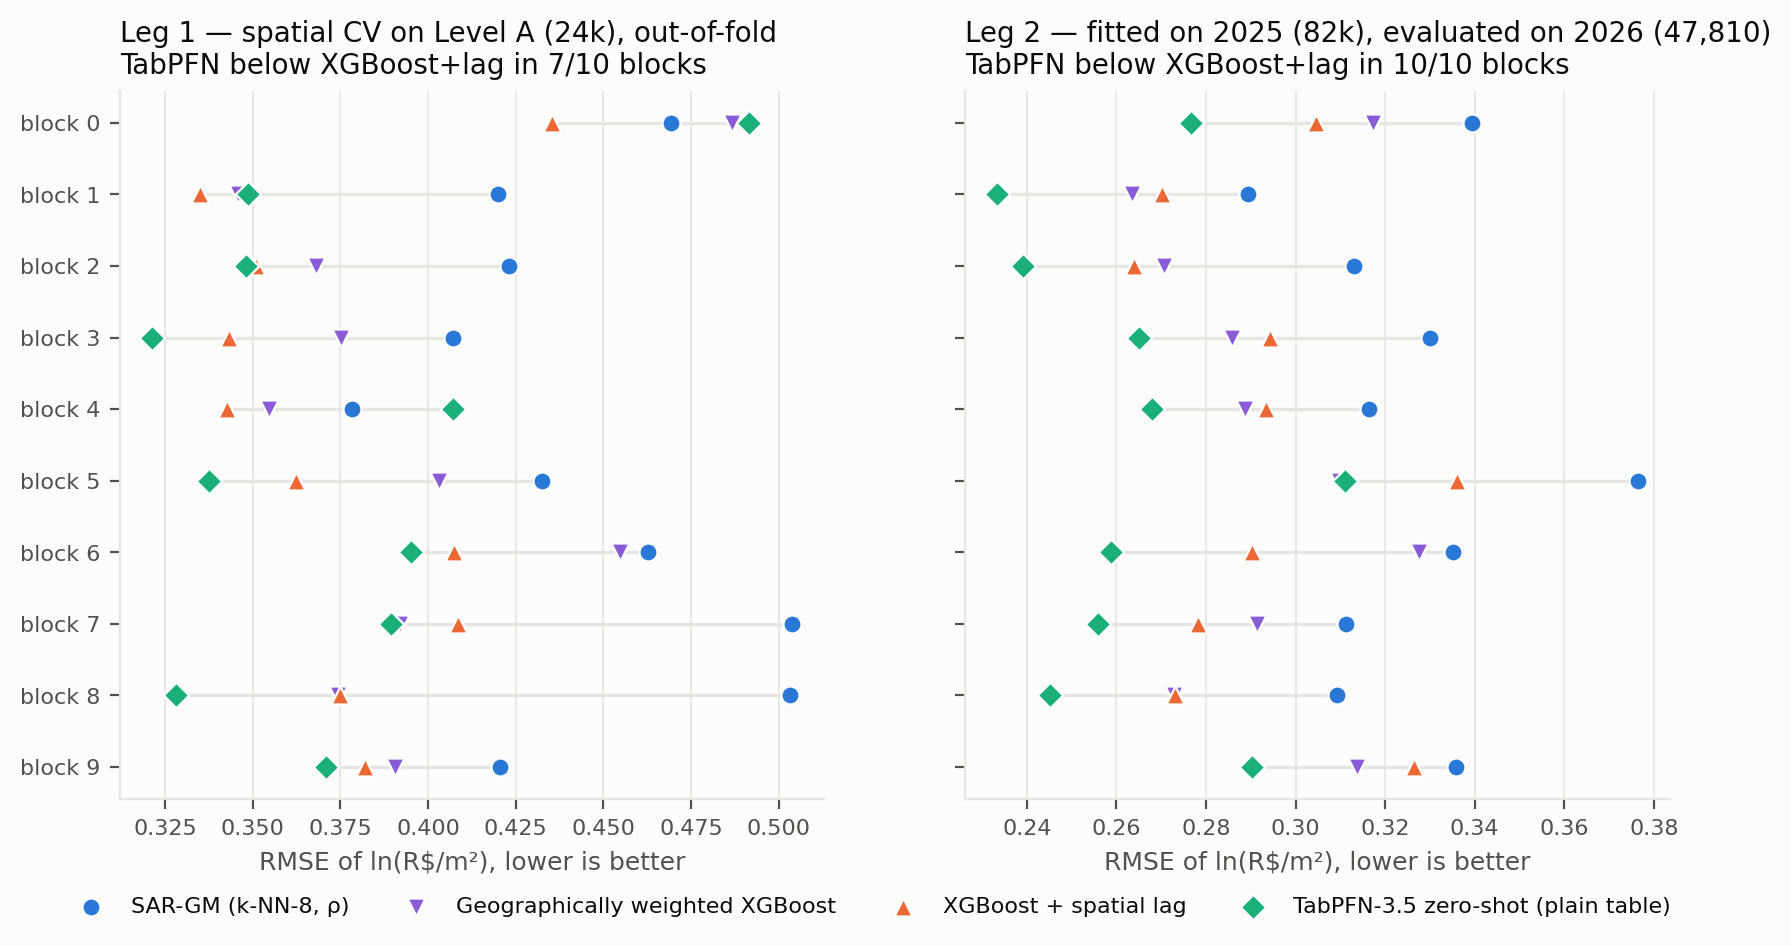
\includegraphics[width=\textwidth]{fig2_per_block_rmse.png}
\caption{RMSE por bloco. Painel esquerdo: validação cruzada por blocos no Nível A (perna 1),
onde o TabPFN-3.5 empata com o XGBoost+defasagem; painel direito: o teste fora do tempo de 2026
com os modelos ajustados na base completa de 2025 (perna 2), onde ele fica abaixo do
XGBoost+defasagem em todos os blocos.}
\label{fig:perblock}
\end{figure}

\begin{figure}[t]
\centering
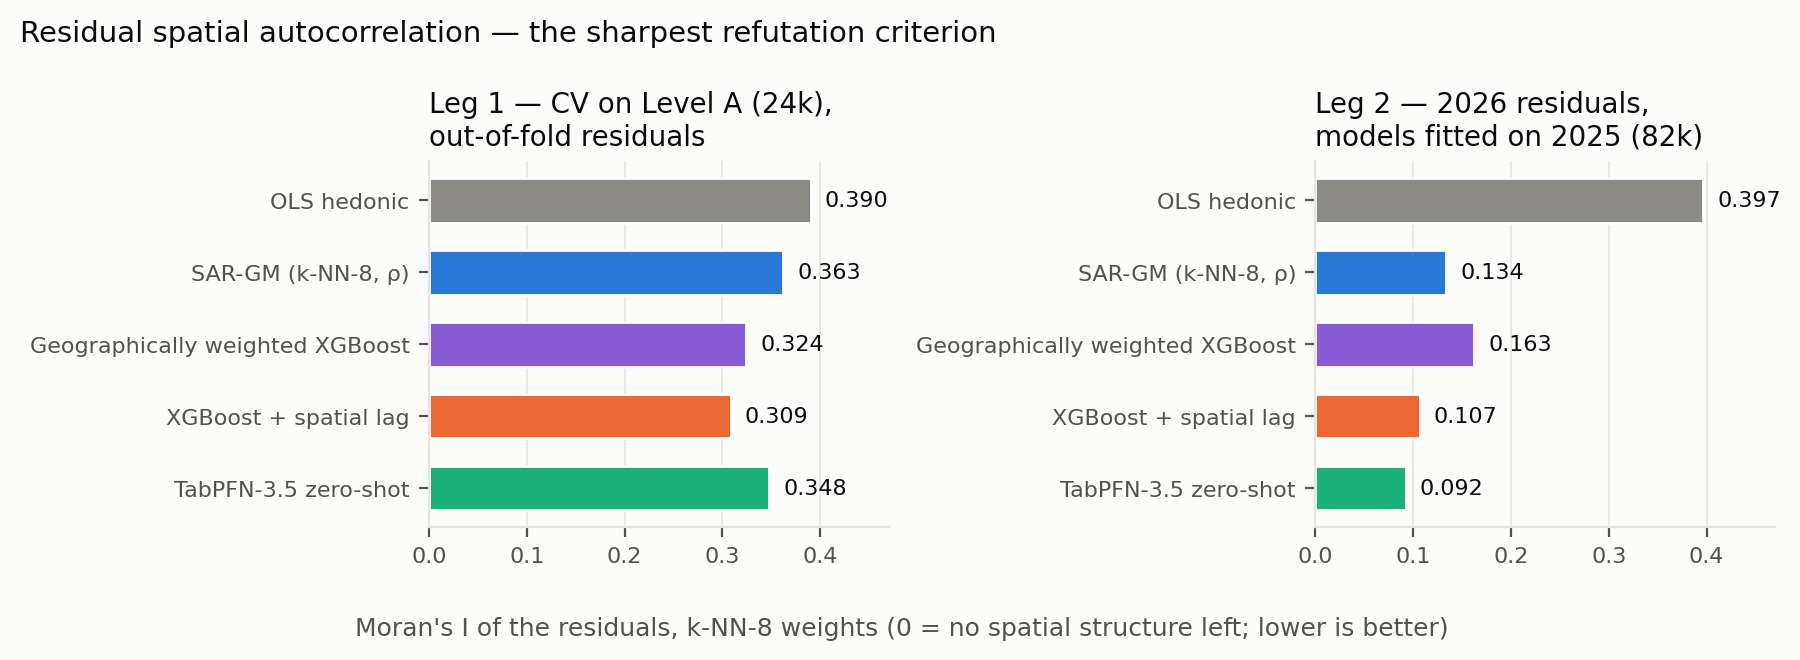
\includegraphics[width=0.9\textwidth]{fig5_moran.png}
\caption{$I$ de Moran dos resíduos, o critério de refutação mais afiado. Painel esquerdo: a
validação por blocos (perna 1), onde o modelo de tabela crua deixa mais estrutura espacial que
qualquer dos dois XGBoost --- a refutação parcial; painel direito: 2026 (perna 2), onde ele
deixa a menor estrutura entre os cinco modelos.}
\label{fig:moran}
\end{figure}

\begin{figure}[t]
\centering
\begin{subfigure}[t]{0.55\textwidth}
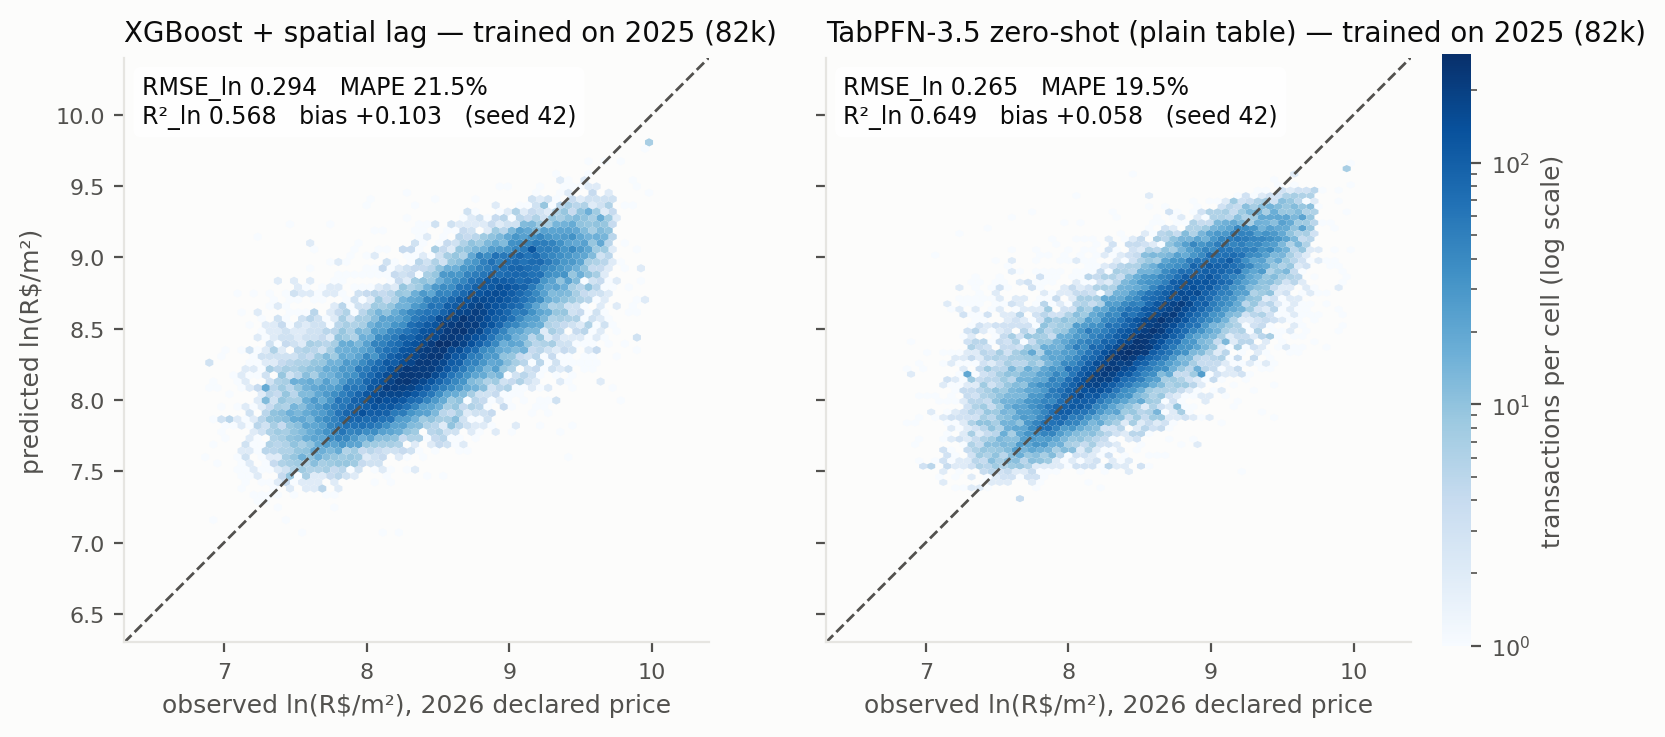
\includegraphics[width=\textwidth]{fig3_pred_vs_obs_2026.png}
\caption{Previsto contra observado, 2026.}
\end{subfigure}\hfill
\begin{subfigure}[t]{0.43\textwidth}
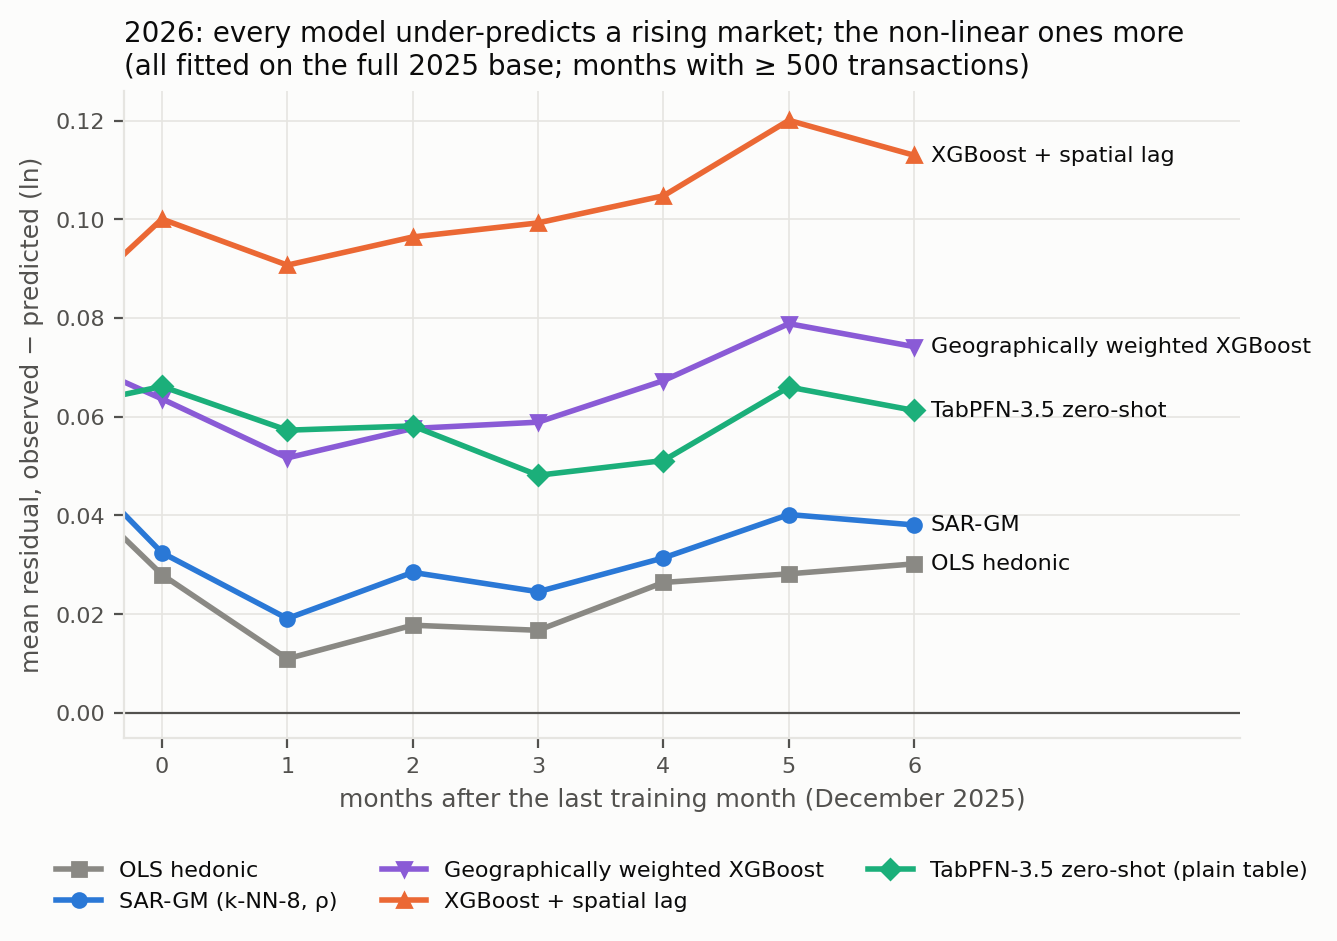
\includegraphics[width=\textwidth]{fig4_months_ahead_bias.png}
\caption{Resíduo médio por mês à frente.}
\end{subfigure}
\caption{O mercado em alta de 2026: todos os modelos subestimam, os aprendizes não lineares
mais.}
\label{fig:bias}
\end{figure}

\textbf{A limitação que merece registro.} Todos os modelos subestimam 2026, um mercado em alta,
e os não lineares mais (viés de $+0{,}04$ a $+0{,}10$ em ln, contra $+0{,}02$ a $+0{,}03$ do
OLS e do SAR): as árvores e o TabPFN seguram o último nível observado do índice do mês em vez
de extrapolar a tendência (Figura~\ref{fig:bias}). A prática de avaliação aplicaria um índice
de preços; aqui o viés é reportado, não corrigido.

\subsection{Robustez: apenas transações financiadas}
\label{sec:robust}

As transações financiadas carregam uma avaliação bancária e são os preços mais limpos da base.
As duas pernas foram rodadas de novo apenas sobre elas: 7.211 das 24.000 linhas do Nível A para
a validação por blocos, as mesmas linhas ajustadas uma vez e avaliadas nas 20.052 transações
financiadas de 2026.

\begin{table}[h]
\centering\small
\caption{As duas pernas apenas nas transações financiadas (semente 42).}
\label{tab:fin}
\footnotesize
\begin{tabular}{lcccccc}
\toprule
Modelo & VC RMSE & VC MAPE & VC $I$ & 2026 RMSE & 2026 MAPE & 2026 $I$ \\
\midrule
Hedônico por OLS & 0,354 & 28,5\% & 0,343 & 0,343 & 26,5\% & 0,491 \\
SAR de defasagem & 0,344 & 28,1\% & 0,342 & 0,286 & 22,0\% & 0,297 \\
XGBoost + defasagem & 0,286 & 23,0\% & 0,327 & 0,221 & 16,7\% & 0,160 \\
TabPFN-3.5, \emph{zero-shot} & \textbf{0,269} & \textbf{21,1\%} & \textbf{0,279} & \textbf{0,207} & \textbf{15,3\%} & \textbf{0,143} \\
\bottomrule
\end{tabular}
\end{table}

Preços mais limpos reduzem todos os erros e deixam inalterado o ranking de um ano à frente. Na
validação por blocos, o modelo de tabela crua passa à frente do XGBoost+defasagem ($\Delta$RMSE
$= -0{,}017$ $[-0{,}032;\ -0{,}003]$, $p = 0{,}049$, 8 de 10 blocos contra a semente 42 dele;
9 de 10 contra as sementes 43 e 44) e a refutação parcial do critério de resíduos não
reaparece: ele deixa menos estrutura espacial que o XGBoost espacial nas duas pernas ($0{,}279$
contra $0{,}327$--$0{,}340$ na VC). Os resultados principais não dependem das compras à vista
retidas pelo filtro de subdeclaração; se algo, os preços à vista, mais ruidosos, são onde o
aprendiz explicitamente espacial se segura. O XGBoost geograficamente ponderado não foi rodado
de novo neste subconjunto.

\subsection{O que carrega a localização}
\label{sec:carriers}

A análise principal entrega ao modelo dois números. O formulário do ITBI também declara a
localização como nomes --- o CEP e um campo livre de bairro --- e descreve o imóvel em
palavras. Quatro variantes de entrada, rodadas sob protocolo idêntico e com as
\emph{baselines} intocadas, perguntam o que o modelo está de fato lendo. Cada uma foi
pré-registrada com uma expectativa na \emph{docstring} do módulo
\texttt{src/model\_tabpfn.py} antes da rodada; as expectativas, e onde falharam, são reportadas
junto com os resultados.

\paragraph{O CEP no lugar das coordenadas.} O CEP (\emph{Código de Endereçamento Postal}) tem
oito dígitos e, em São Paulo, costuma corresponder a uma rua ou a um trecho de rua: 10.022
valores distintos nas 24.000 linhas do Nível A e 15.938 na base completa de 2025, e nada na
coluna diz qual código fica ao lado de qual. A variante remove latitude, longitude e a
distância à estação (calculada a partir delas) e põe o código bruto no lugar, como texto --- a
única informação espacial que o modelo recebe, contra \emph{baselines} que mantêm todos os seus
insumos espaciais. A expectativa escrita era que o código recuperasse menos da metade do
caminho entre o piso sem localização e o modelo com coordenadas, e perdesse para o
XGBoost+defasagem nas duas pernas.

\begin{table}[h]
\centering\small
\caption{O CEP no lugar das coordenadas (\emph{zero-shot}, semente 42) contra a tabela crua.
RMSE no logaritmo do valor unitário $\cdot$ $I$ de Moran dos resíduos; as entradas da perna 1
da tabela crua são faixas sobre as três sementes. As \emph{baselines} são as das
Tabelas~\ref{tab:cv} e~\ref{tab:oot}.}
\label{tab:postal}
\footnotesize
\begin{tabular}{lccc}
\toprule
Entrada do TabPFN-3.5 & Perna 2, 24k $\to$ 2026 & Perna 2, 82k $\to$ 2026 & Perna 1 (VC) \\
\midrule
Apenas o CEP & 0,277 $\cdot$ 0,129 & 0,268 $\cdot$ 0,091 & 0,457 $\cdot$ 0,502 \\
Latitude e longitude & 0,275 $\cdot$ 0,122 & 0,265 $\cdot$ 0,092 & 0,391--0,394 $\cdot$ 0,342--0,348 \\
\bottomrule
\end{tabular}
\end{table}

Um ano à frente, a expectativa falhou na direção favorável ao modelo: o rótulo faz o trabalho
das coordenadas. O modelo só-CEP recupera $94$--$97\%$ do caminho entre seu piso sem
localização ($0{,}352$ no Nível A, $0{,}327$ na base completa) e o modelo com coordenadas, e
vence cada semente de cada \emph{baseline} espacial: o XGBoost+defasagem por $-0{,}011$ (24k) e
$-0{,}014$ (82k) contra a melhor semente dele, em 10 de 10 blocos; o geograficamente ponderado
por $-0{,}036$ e $-0{,}029$ (10 e 9 de 10); o SAR por $-0{,}069$ e $-0{,}057$ (10 de 10;
Wilcoxon $p = 0{,}002$ em toda parte, $p = 0{,}004$ na linha de 9 de 10). Ele também deixa
menos autocorrelação residual que os três --- e o $I$ de Moran é calculado sobre a matriz
$k$-NN-8 das próprias coordenadas que foram negadas ao modelo. O resultado não é uma consulta
de preço por código: nas transações de 2026 cujo código nunca ocorre na base de treino
($22\%$ delas contra o Nível A, $9\%$ contra a base completa), o modelo ainda recupera $97\%$ e
$96\%$ do sinal de localização, quase tanto quanto nos códigos já vistos ($98\%$ e $94\%$).
Tampouco é o código informação mais rica do que as \emph{baselines} tinham: dentro do TabPFN
ele chega a $0{,}004$ do par de coordenadas e, somado a elas, nada muda (abaixo); o XGBoost
tinha as coordenadas \emph{e}, por cima, uma defasagem, eixos rotacionados e a distância à
estação.

Onde o rótulo para é numa parte da cidade nunca vista. Na perna 1 os códigos de um bloco
deixado de fora estão ausentes do treino por construção ($97$--$100\%$), e ali o código carrega
pior do que nada: o modelo cai abaixo do próprio piso sem localização ($0{,}457$ contra
$0{,}440$), perde para o XGBoost+defasagem no erro agregado ($+0{,}069$ a $+0{,}072$, 4 de 10
blocos) e deixa a maior autocorrelação espacial de qualquer modelo do estudo ($I = 0{,}502$)
--- um bloco inteiro de códigos desconhecidos é precificado como uma única incógnita, e o erro
se desloca em bloco. Esta perna se comportou como a expectativa escrita dizia, e pior.
Coordenadas extrapolam para um distrito não visto; um rótulo, não. Por que códigos nunca
vistos, em meio a códigos conhecidos, ainda funcionam não está resolvido; a hipótese principal
é a ordem: os CEPs brasileiros são atribuídos geograficamente, de modo que códigos vizinhos em
geral significam ruas vizinhas, e o teste que decidiria a questão (uma bijeção aleatória fixa
dos códigos, que destrói a ordem e preserva as identidades) está desenhado, mas não foi
executado.

\paragraph{O endereço somado às coordenadas.} Acrescentar o CEP e o campo de bairro à tabela
crua, tal como preenchidos, move o RMSE em menos de $0{,}006$ em qualquer direção em todos os
testes, o MAPE em no máximo $0{,}3$ ponto e o $I$ de Moran residual em no máximo $0{,}008$; a
margem sobre o XGBoost+defasagem fica onde estava. Duas colunas numéricas cruas já carregam o
que o endereço carrega. Uma observação lateral é reportada sem explicação: com os dois nomes na
tabela, a subestimação média de 2026 cai de $+0{,}055$ para $+0{,}045$ em ln no Nível A e de
$+0{,}058$ para $+0{,}043$ na base completa, com o RMSE parado.

\paragraph{A unidade e o edifício como escritos.} O complemento da unidade do formulário
(\texttt{AP 201 E 3VGS}: apartamento 201 com três vagas) e o campo \emph{Referência}, que em
geral nomeia o edifício (\texttt{EDIFICIO THE PARK}), entram como texto bruto ao lado das
coordenadas; nada é interpretado. A expectativa escrita era de um ganho pequeno, no máximo, um
ano à frente, onde os mesmos edifícios voltam a vender, com a perna 1 como controle
quase negativo. A expectativa errou o lugar.

\begin{table}[h]
\centering\small
\caption{O texto da unidade e do edifício somado à tabela crua (\emph{zero-shot}, semente 42).
$\Delta$ é texto $-$ tabela crua, IC 95\% por \emph{bootstrap} de blocos; blocos vencidos pela
variante com texto.}
\label{tab:text}
\scriptsize\setlength{\tabcolsep}{2.8pt}
\begin{tabular}{lccc}
\toprule
 & Tabela crua & $+$ texto da unidade e do edif. & $\Delta$RMSE [IC 95\%] $\cdot$ blocos \\
\midrule
Perna 1, VC por blocos & 0,3938 $\cdot$ 32,2\% $\cdot$ $I$ 0,348 & 0,3835 $\cdot$ 30,8\% $\cdot$ 0,331 & $-0{,}0103$ $[-0{,}0161;\ -0{,}0031]$ $\cdot$ 8/10 \\
Perna 2, 24k $\to$ 2026 & 0,2750 $\cdot$ 20,4\% $\cdot$ 0,122 & 0,2750 $\cdot$ 20,6\% $\cdot$ 0,122 & $+0{,}0000$ $[-0{,}0011;\ +0{,}0010]$ $\cdot$ 6/10 \\
Perna 2, 82k $\to$ 2026 & 0,2649 $\cdot$ 19,5\% $\cdot$ 0,092 & 0,2610 $\cdot$ 19,2\% $\cdot$ 0,086 & $-0{,}0039$ $[-0{,}0049;\ -0{,}0031]$ $\cdot$ 10/10 \\
\bottomrule
\end{tabular}
\end{table}

O maior ganho está no distrito nunca visto, contra cada uma das três sementes da tabela crua
($-0{,}007$ a $-0{,}010$, todos os intervalos fora do zero). Ali o texto transforma o empate
com o XGBoost geograficamente ponderado em vitória ($-0{,}023$ a $-0{,}026$, 9 de 10 blocos,
$p = 0{,}027$), mantém um empate pendendo para o TabPFN contra o XGBoost+defasagem e entrega o
menor MAPE de qualquer modelo daquela perna ($30{,}8\%$). Não é casamento de cadeias de
caracteres: $92\%$ dos nomes de edifício de um bloco deixado de fora nunca ocorrem nas dobras
de treino, e complementos nunca vistos como texto exato ganham tanto quanto os já vistos
($-0{,}014$ contra $-0{,}013$). O ganho está nos formulários que mencionam vaga ($-0{,}034$),
unidades comerciais ($-0{,}023$) ou um edifício nomeado ($-0{,}017$): o que transfere para um
distrito não visto é o que as palavras dizem, não o edifício que apontam. O critério dos
resíduos estreita, mas permanece: o $I$ de Moran cai de $0{,}348$ para $0{,}331$, ainda acima
das duas variantes de XGBoost.

\paragraph{\emph{Thinking} com os blocos como grupos.} O modo \emph{thinking} pode separar sua
validação interna por uma coluna de agrupamento; com o bloco espacial como grupo, a validação
interna passa a deixar distritos inteiros de fora, como a perna 1 faz. Contra o
\emph{thinking} sem grupos, a mudança na perna 1 é $+0{,}0038$ $[-0{,}0055;\ +0{,}0149]$ (3 de
10 blocos) e o $I$ residual vai de $0{,}342$ a $0{,}350$: o agrupamento não fecha a lacuna. Um
ano à frente ele ganha $0{,}0014$ $[-0{,}0021;\ -0{,}0007]$ no RMSE e reduz a subestimação
média de $+0{,}055$ para $+0{,}043$, mas ali o rótulo do bloco também informa ao modelo a que
parte da cidade pertence uma linha de 2026, de modo que o pequeno ganho não é um efeito puro de
calibração. Num distrito não visto, o limite é de informação, não de desenho de validação: o
texto move a perna 1, o agrupamento não.

\subsection{Explicando uma estimativa}

\begin{figure}[t]
\centering
\begin{subfigure}[t]{0.49\textwidth}
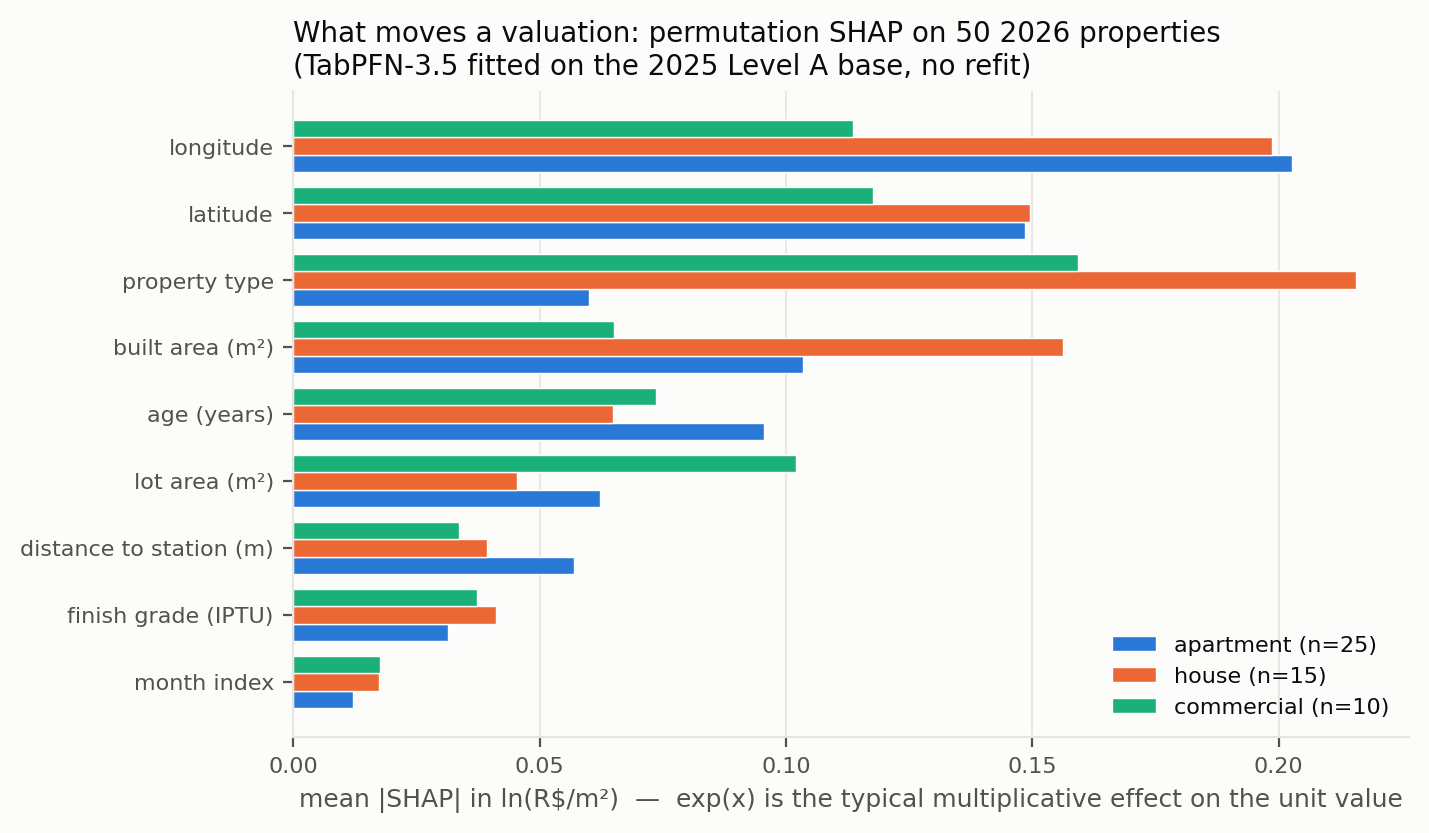
\includegraphics[width=\textwidth]{fig6_shap_importance.png}
\caption{Média de $|$SHAP$|$ por atributo e tipo.}
\end{subfigure}\hfill
\begin{subfigure}[t]{0.49\textwidth}
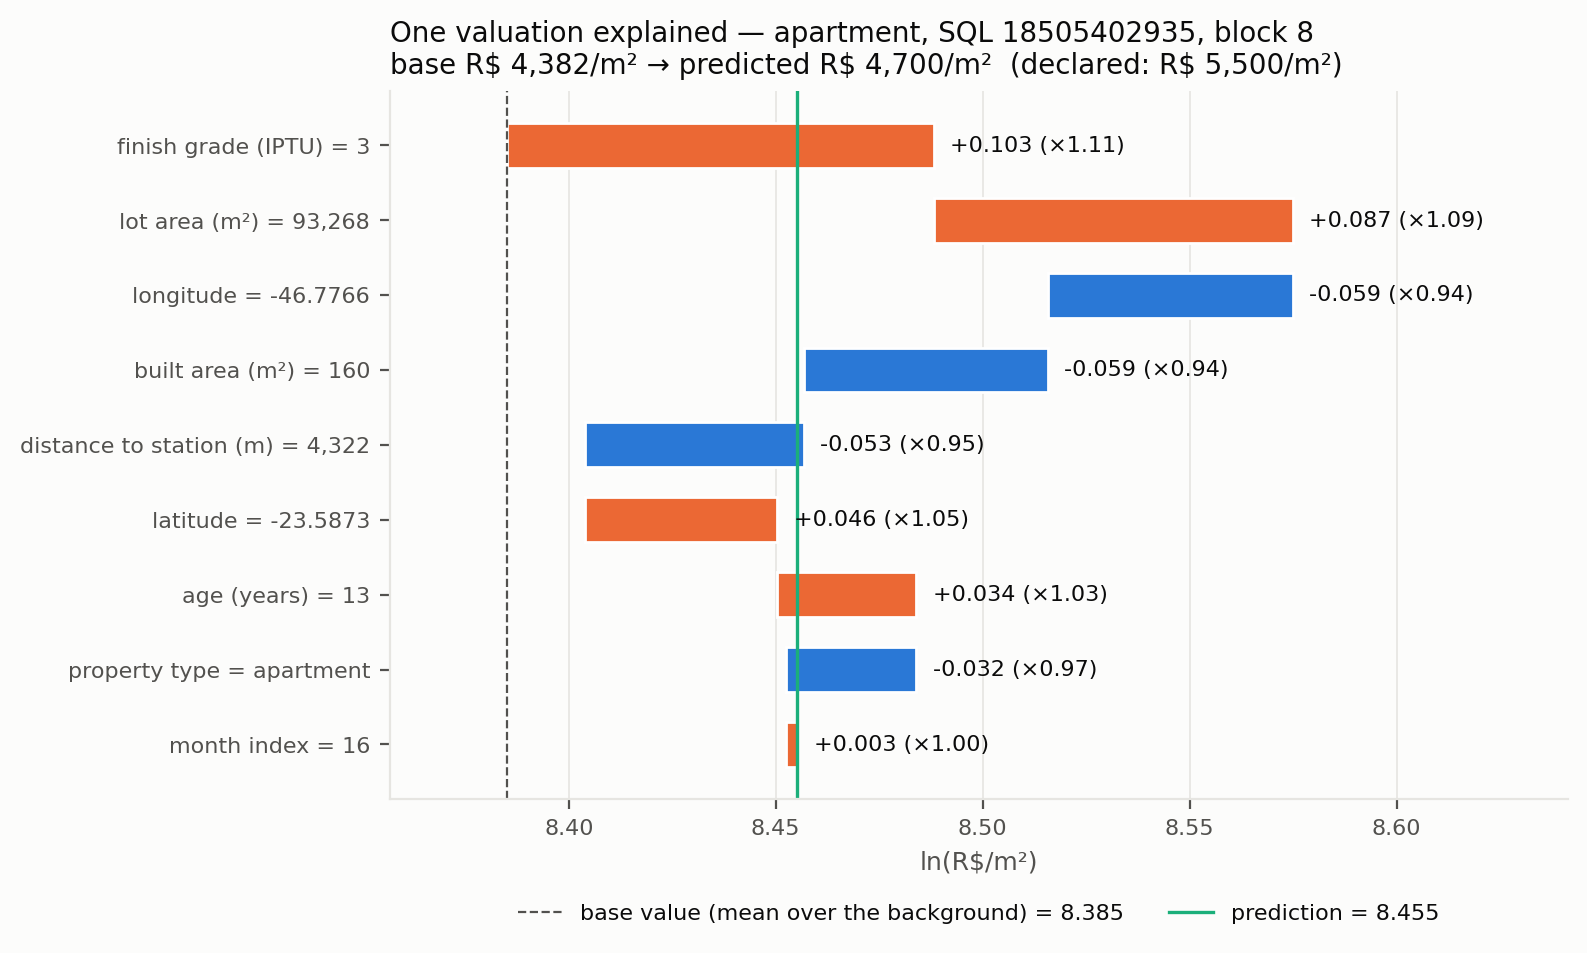
\includegraphics[width=\textwidth]{fig8_shap_waterfall.png}
\caption{Uma avaliação, do valor-base à estimativa.}
\end{subfigure}
\caption{SHAP por permutação em 50 transações de 2026 (\emph{masker} independente, fundo de 20
linhas), com o modelo recarregado de seu registro em cache. Valores na escala logarítmica;
$e^{\text{SHAP}}$ é o multiplicador sobre o valor unitário.}
\label{fig:shap}
\end{figure}

O avaliador que assina um laudo precisa dizer por quê. Como o modelo é servido por uma API, a
explicação é o SHAP por permutação, agnóstico ao modelo \citep{lundberg2017shap}, sobre 50
transações estratificadas de 2026 que o modelo nunca viu, com cada uma das 27.217 linhas
previstas em cache para reprodução \emph{offline}. Recarregado de seu registro em cache, o
modelo reproduz as predições que está explicando (RMSE de $0{,}296$ em ln nas 50 linhas), de
modo que as atribuições descrevem a rodada que foi avaliada. Longitude (média de $|$SHAP$|$ de
$0{,}184$, um multiplicador típico de $\times 1{,}20$ sobre o valor unitário) e latitude
($0{,}143$, $\times 1{,}15$) são os dois insumos mais fortes, à frente da tipologia
($0{,}127$), da área construída ($0{,}112$) e da idade ($0{,}082$). As direções coincidem com a
experiência do avaliador: idade e distância à estação puxam o valor unitário para baixo, o
padrão construtivo empurra para cima, áreas construídas maiores reduzem o preço por metro
quadrado. As duas coordenadas cruas carregam, dentro do modelo, o sinal que as \emph{baselines}
codificam com uma matriz de pesos --- e a Seção~\ref{sec:carriers} mostra que o que elas
carregam, dentro de um mercado observado, é a localização como identificador, não geometria.

\section{Discussão}
\label{sec:discussion}

Lidas juntas, as duas pernas traçam uma linha. Dentro de um mercado que o modelo viu --- a
mesma cidade, um a sete meses à frente ---, o aprendizado em contexto sobre 24 mil a 82 mil
linhas recupera a estrutura de vizinhança de duas colunas cruas e precifica melhor do que os
modelos construídos para codificá-la, por todos os critérios pré-registrados, autocorrelação
residual incluída. A variante com o CEP afia a leitura: dentro desse mercado, o modelo não
precisa de geometria alguma, apenas de um identificador fino de localização, e precifica
códigos nunca vistos, em meio a códigos conhecidos, quase tão bem quanto os conhecidos. Do
outro lado da linha, num distrito sem vendas na base de treino, o identificador colapsa, as
coordenadas ainda extrapolam, e a defasagem espacial explícita ganha o seu sustento no critério
dos resíduos: a refutação parcial da perna 1 é o preço medido de não modelar o espaço quando o
bloco de teste é terreno novo. Esse preço encolhe com mais informação --- o texto livre do
formulário reduz a lacuna e o erro --- e não aparece nos preços financiados, auditados pelo
banco, contra o XGBoost+defasagem; na análise principal, porém, ele não desaparece, e é
reportado como encontrado.

O único erro sistemático comum a todos os modelos é a tendência. Todos subestimam o mercado em
alta de 2026, os aprendizes não lineares mais ($+0{,}04$ a $+0{,}10$ em ln, contra $+0{,}02$ a
$+0{,}03$ dos modelos lineares), porque as árvores e o modelo de fundação seguram o último
nível observado do índice do mês em vez de extrapolá-lo. A prática de avaliação corrige isso
com um índice de preços como rotina; nenhuma correção foi aplicada aqui, para que a comparação
permaneça entre modelos tal como ajustados. O viés diz respeito ao nível, não à localização: os
mapas de resíduos e o $I$ de Moran, que a tendência desloca uniformemente, continuam separando
os modelos.

O balanço de engenharia é curto. O SAR precisa de uma matriz de pesos por dobra; o XGBoost
espacial, de uma defasagem interna à dobra, eixos rotacionados e 30 tentativas de ajuste
aninhado (cerca de 15 minutos de calibração na base completa); o XGBoost geograficamente
ponderado, de 1.000 modelos locais e uma busca interna de banda e mistura (cerca de dez
minutos). O TabPFN-3.5 precisa da tabela: um ajuste de 9 a 15 segundos e, onde um CEP já está
no formulário, nem de um geocodificador. Para a avaliação em massa sob a norma brasileira
NBR 14653-2, seguem-se duas consequências. Os graus de precisão da norma são definidos sobre
estimativas intervalares, e o modelo devolve quantis preditivos sem engenharia adicional ---
eles estão em cache para todos os ajustes \emph{zero-shot} deste estudo, e a análise de
cobertura é o passo seguinte natural. E a exigência de fundamentação da norma pode ser
atendida, em parte, por atribuição agnóstica ao modelo: as direções do SHAP acima são as que um
avaliador defenderia.

Os limites da evidência são estes. As coordenadas são centroides de quadra fiscal, de modo que
a localização é resolvida na quadra e todas as transações de uma mesma quadra coincidem; um
\emph{jitter} determinístico submétrico desfaz os empates apenas para as matrizes de pesos. Os
preços são autodeclarados; o filtro de subdeclaração remove o acúmulo detectável, não o
fenômeno, e a robustez só-financiados limita o seu efeito. O estudo cobre uma cidade e um
período, e o modelo de fundação é servido por uma API: seus internos não são inspecionáveis
(daí não haver atribuição exata por linha para a cabeça de regressão) e a versão hospedada pode
mudar, embora os pesos estejam publicados para uso em pesquisa e cada resposta da API esteja em
cache. As variantes de entrada do TabPFN rodaram com uma única semente; a dispersão entre
sementes da tabela crua na perna 1 ($0{,}003$ em ln) fica muito abaixo de todas as margens da
perna 2, mas os empates da perna 1 devem ser lidos com essa largura em mente. O XGBoost
geograficamente ponderado é uma aproximação do estimador publicado --- modelos locais em 1.000
pontos de regressão em vez de em cada linha de treino, hiperparâmetros locais compartilhados,
piso de banda de 50 vizinhos que a busca interna escolheu em 8 de 10 dobras ---, defensável nos
termos da própria regressão geograficamente ponderada e balizada pela sensibilidade de banda
reportada acima. O teste do CEP embaralhado, que resolveria por que códigos não vistos
funcionam, está desenhado, não executado.

\section{Conclusão}
\label{sec:conclusion}

A hipótese era que um modelo de fundação tabular recebendo as coordenadas como duas colunas
numéricas simples prevê preços espacialmente correlacionados tão bem quanto, ou melhor que,
modelos que codificam a dependência espacial explicitamente, e ela foi posta em risco contra
quatro desses modelos, sobre 130.000 preços de transação declarados, com os critérios de
refutação escritos antes. Um ano à frente, dentro do mercado observado, a hipótese sobrevive a
todos os critérios nas duas escalas de treino: erro agregado menor que o do SAR, do XGBoost com
defasagem espacial e do XGBoost geograficamente ponderado, vitórias em pelo menos 9 dos 10
blocos espaciais contra cada semente de cada oponente, e a menor autocorrelação espacial
residual dos cinco modelos --- um veredito que se mantém mesmo quando as coordenadas são
substituídas por um CEP bruto. Num distrito nunca visto, ela empata com as duas variantes de
XGBoost no erro, vence o SAR e é parcialmente refutada no critério dos resíduos, deixando mais
estrutura espacial que qualquer dos dois XGBoost; o texto livre do formulário estreita essa
lacuna e o subconjunto financiado a dissolve contra o XGBoost+defasagem, mas na análise
principal ela permanece. O veredito poderia mudar em outro lugar: outra cidade ou mercado,
ofertas em vez de preços declarados, uma versão do modelo com atribuição por linha na
regressão, ou o teste do código embaralhado são os experimentos que o moveriam. Como está, para
a avaliação em massa dentro de um mercado com histórico de vendas, o preditor mais forte desta
comparação é o modelo de fundação com a tabela crua --- sem matriz de pesos, sem defasagem, sem
atributos de vizinhança, um ajuste de quinze segundos.

\section*{Reprodutibilidade e disponibilidade dos dados}
Código, dados limpos, respostas do modelo em cache e todos os números deste artigo estão em
\url{https://github.com/abenvenho/tabpfn-itbi-sp} (Apache-2.0); todos os dados de origem são
públicos (dados abertos municipais sob a Lei de Acesso à Informação). O \emph{pipeline} foi
reexecutado a partir de um clone limpo: as três bases foram reconstruídas byte a byte idênticas
a partir das planilhas públicas brutas, e as rodadas de fumaça e de \emph{baseline} devolveram
os números documentados. Todo número citado neste manuscrito é conferido contra os resultados
versionados por \texttt{paper/check\_numbers.py}.

\section*{Agradecimentos}
Este estudo foi realizado como entrada no \emph{hackathon} TabPFN-3.5 da Prior Labs, cujos
créditos de API para participantes custearam as rodadas do modelo.

\paragraph{Declaração de assistência de IA.} O código deste estudo foi desenvolvido com a
assistência de ferramentas de IA em nuvem --- Claude (modelos Fable e Opus) e ChatGPT (Astra)
--- e dos modelos executados localmente Qwen 3.8 Next Flash e Qwen 3 Coder Next. As
ferramentas de nuvem também auxiliaram na redação, tradução, pesquisa bibliográfica, geração de
figuras e revisão de texto. O desenho experimental, as decisões metodológicas, a análise dos
resultados e as conclusões são do autor, que revisou e assume a responsabilidade por todo o
conteúdo.

\bibliographystyle{plainnat}
\bibliography{refs}

\appendix

\section{XGBoost geograficamente ponderado: piloto de viabilidade}
\label{app:gxgb}

A implementação publicada (\texttt{geoxgboost}) calibra um XGBoost local, com sua própria busca
em grade, em cada linha de treino, sobre uma matriz densa de distâncias $n \times n$. Um piloto
com 200 linhas e um candidato de banda levou 18,7~s ($0{,}093$~s por unidade espacial), o que
extrapola para cerca de meia hora por candidato de banda por dobra nas 19.117 linhas de treino
de uma dobra do Nível A, cerca de dois dias para dez candidatos em dez dobras, e 2,9~GB de
matriz de distâncias por dobra na máquina do estudo (2 vCPU, 7~GB de RAM;
\texttt{results/gxgb\_timing\_pilot.json}). A aproximação por pontos de regressão da
Seção~\ref{sec:methods} preserva o estimador --- modelos locais, pesos bi-quadrados, mistura
com um modelo global, escolha aninhada da banda --- em cerca de um minuto por ajuste e dez por
calibração.

\section{Hiperparâmetros e configurações dos modelos}
\label{app:hparams}

\paragraph{XGBoost com atributos espaciais.} Optuna aninhado, 30 tentativas TPE por dobra
externa, \emph{leave-one-block-out} interno sobre os blocos de treino, parada antecipada com
até 3.000 rodadas. Espaço de busca: taxa de aprendizado $0{,}01$--$0{,}2$ (log), profundidade
máxima $3$--$10$, peso mínimo por folha $1$--$50$ (log), \emph{subsample} $0{,}5$--$1$,
\emph{colsample\_bytree} $0{,}4$--$1$, $\lambda$ $10^{-3}$--$30$ (log), $\alpha$
$10^{-3}$--$10$ (log), $\gamma$ $10^{-4}$--$1$ (log). Selecionados para o ajuste fora do tempo
na base completa (semente 42): taxa de aprendizado $0{,}049$, profundidade $7$, peso mínimo
$2{,}0$, \emph{subsample} $0{,}89$, \emph{colsample} $0{,}56$, $\lambda$ $0{,}0033$, $\alpha$
$0{,}0041$, $\gamma$ $0{,}0031$, $398$ rodadas; RMSE interno $0{,}351$; tempo de calibração
$901$~s (\texttt{results/xgb\_params\_*.json}).

\paragraph{XGBoost geograficamente ponderado.} $M = 1.000$ pontos de regressão ($K$-médias das
coordenadas de treino); modelos locais com hiperparâmetros compartilhados ($300$ rodadas, taxa
de aprendizado $0{,}05$, profundidade $4$); modelo global com $800$ rodadas, taxa $0{,}05$,
profundidade $6$; uma consulta é prevista pela média, com pesos inversos à distância, de seus
$3$ modelos locais mais próximos, combinada por $\alpha$. Banda $k$ e $\alpha$ por validação
cruzada interna aninhada por blocos, grades na Seção~\ref{sec:methods}; escolhidos no Nível A:
$k$ por dobra entre 40 e 176 com $\alpha = 0{,}5$ (perna 1), $k = 50$ (perna 2, 24k) e
$k = 342$ (perna 2, 82k), $\alpha = 0{,}5$ em toda parte
(\texttt{results/gxgb\_params\_*.json}).

\paragraph{TabPFN-3.5.}\sloppy{} Modelo hospedado (\texttt{tabpfn-client} 0.6.0), criado por
\texttt{create\_default\_for\_version} com a versão \texttt{"v3.5"}; cabeça de regressão, \emph{zero-shot} salvo
indicação. Modo \emph{thinking}: \texttt{thinking\_effort} médio ou alto,
\texttt{thinking\_metric = "rmse"}, tempo-limite de 2.400~s; a variante agrupada passa o bloco
espacial como \texttt{group\_col}. Os ajustes com as 82.187 linhas usam
\texttt{ignore\_pretraining\_limits}. Quantis preditivos são solicitados e armazenados em cache
em todo ajuste \emph{zero-shot}. Toda resposta da API fica em cache sob
\texttt{results/tabpfn\_cache/}, de modo que o protocolo completo roda de novo \emph{offline} a
partir das predições em cache.\par\fussy

\end{document}
